\documentclass[a4paper]{article}
\usepackage[utf8]{inputenc}
\usepackage{graphicx}
\graphicspath{ {imgs/} {tables/} }
\usepackage{floatrow}
\usepackage{array}
\usepackage[margin=1in]{geometry}
\usepackage{courier}
\usepackage{etoolbox}
\usepackage[htt]{hyphenat}
\usepackage[dvipsnames,table]{xcolor}
\usepackage{listings}
\usepackage{makecell}
\usepackage{hyperref}
\usepackage{booktabs}
\usepackage{tabularx}
\usepackage{tabulary}
\usepackage{multicol}

\setlength{\columnsep}{2em}

\hypersetup{
    colorlinks=true,
    linkcolor=blue,
    filecolor=magenta,      
    urlcolor=cyan,
}

\newenvironment{mono}{\fontfamily{pcr}\selectfont}{\par}

\renewcommand\theadalign{bc}
\renewcommand\theadfont{\bfseries}
\renewcommand\theadgape{\Gape[4pt]}
\renewcommand\cellgape{\Gape[4pt]}
\definecolor{codegreen}{rgb}{0,0.6,0}
\definecolor{codegray}{rgb}{0.5,0.5,0.5}
\definecolor{codepurple}{rgb}{0.58,0,0.82}
\definecolor{backcolour}{rgb}{0.95,0.95,0.92}

\lstdefinestyle{mystyle}{
    backgroundcolor=\color{backcolour},   
    commentstyle=\color{codegreen},
    keywordstyle=\color{magenta},
    numberstyle=\tiny\color{codegray},
    stringstyle=\color{codepurple},
    basicstyle=\ttfamily\small,
    breakatwhitespace=false,         
    breaklines=true,                 
    captionpos=b,                    
    keepspaces=true,                 
    numbers=left,                    
    numbersep=5pt,                  
    showspaces=false,                
    showstringspaces=false,
    showtabs=false,                  
    tabsize=2
}

\lstset{style=mystyle}

\title{\textbf{GIT Department Of Computer Engineering\\ 
CSE 222/505 - Spring 2020\\
Homework 8 Report \vspace{1in}}}

\author{\textbf{Fatih Kaan Salgır} \\ 
\textbf{171044009}}

\date{}

\begin{document}

\begin{large}

  \maketitle

  \newpage

  \begin{center}
    \textbf{ \\
      \vspace{3cm}
      \Huge{PART 3}
    }
  \end{center}

  \newpage

  \section{Problem Solution Approach}

	First I have read the file to a 2 dimensional boolean \texttt{ArrayList}. Then I have call the recursive \texttt{discover()} method which starts form beginning position and moves through 0's (false) in 2D \texttt{ArrayList}, identify vertexes and create edges. There are some cases to consider in this method. First we cannot simply check if node is visited before checking if it is a vertex. Because in this case some edges would be missing. When we find a vertex, before creating new vertex we must check if we added this vertex to vertices list. To get the vertex we need it's x and y coordinates. Therefore we can use a \texttt{Map} data structure, with keys are coordinates and values are vertices. Another case to consider when new vertex is found is, checking if last vertex is the vertex we found. In this case we will return because vertexes don't have edges to itself. Also I have used \texttt{Set} data structure to store edges to avoid duplicate. 
  \vspace{1em}

	Second step is creating the graph with the edges and the vertices we have found. I have used list graph representation, because by looking the map we can see that graph will be sparse, there are not many edges compare to number of vertices. 
  \vspace{1em}

	For finding the shortest path I have used the dijkstras algorithm. By using the output of dijkstras algorithm I have created a Map structure which consist of source - destination. Searching in this map and putting into a stack gives us reverse of the shortest path. Therefore to obtain shortest path, I have poped the items in the stack and print them out.

  \newpage

  \section{Class Diagrams}

  \begin{figure}[htp]
    \centering
    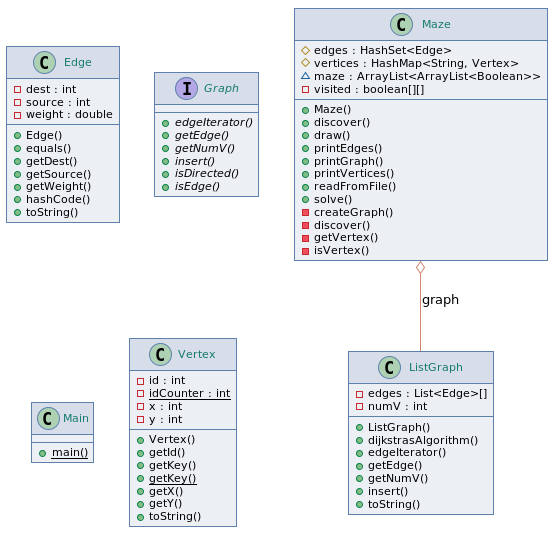
\includegraphics[width=0.9\textwidth]{class-diagram-3}
  \end{figure}

  \newpage

  \section{Test Cases}

  I have created some text cases for some adding and removing operations which is present on my main method as commented out.

  \begin{figure}[htp]
    \centering
    \hspace*{-1.5cm}
    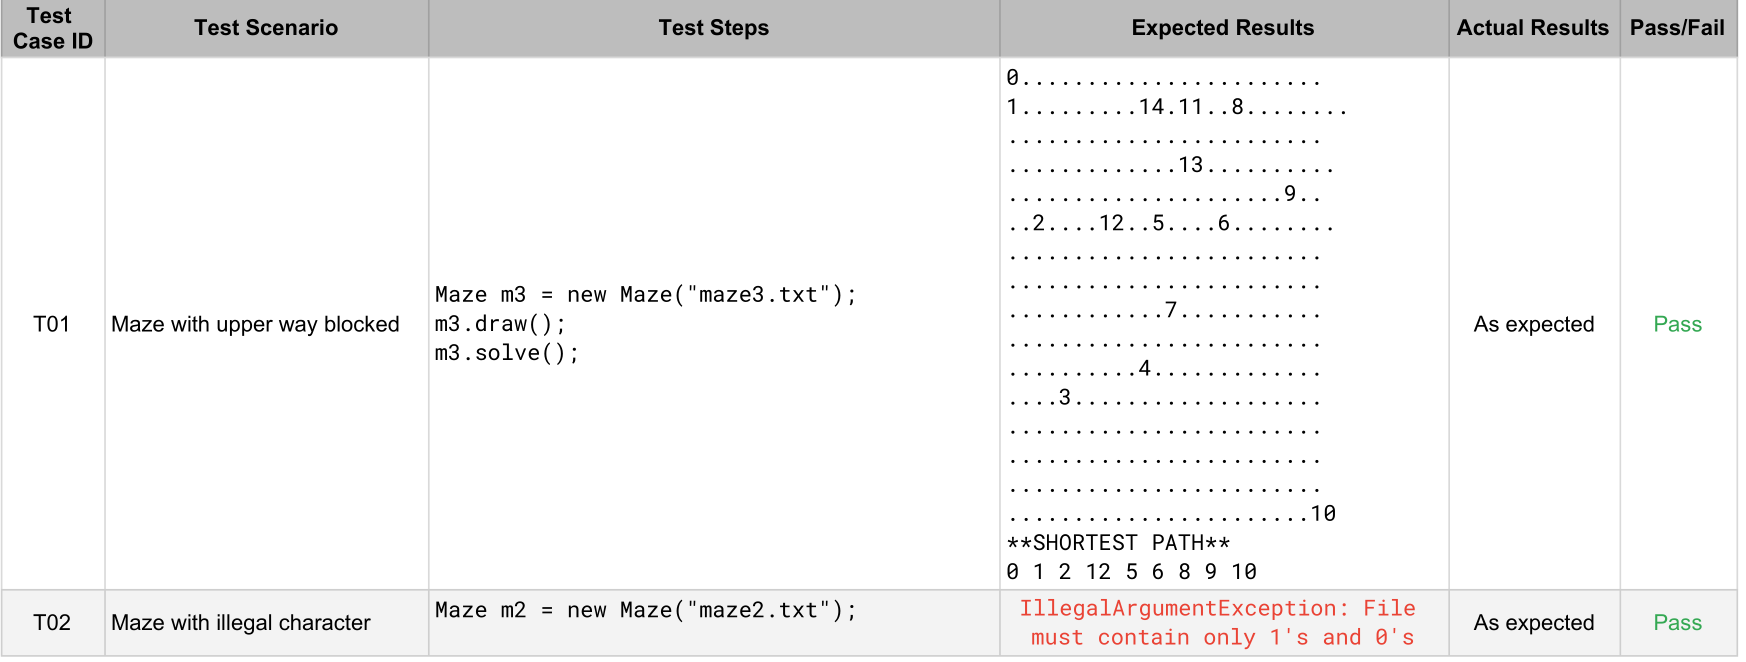
\includegraphics[width=1.20\textwidth]{test-case-3}
  \end{figure}

  \section{Running and Results}

  \begin{lstlisting}[language=Java, caption=Testing methods in main method]
Maze maze = new Maze("maze.txt");
maze.draw();
maze.printVertices();
maze.printEdges();
maze.printGraph();
maze.solve();

System.out.println("T1");
Maze m3 = new Maze("maze3.txt");
m3.draw();
m3.solve();
System.out.println("T2");
Maze m2 = new Maze("maze2.txt");
  \end{lstlisting}

  \newpage

  Output of the test cases;


\begin{lstlisting}[caption=Visual representation of found vertices in maze]
0.......................
1..............8........
........................
.............12..........
.....................9..
..2....11..5....6........
........................
........................
............7...........
........................
..........4.............
....3...................
........................
........................
........................
.......................10
\end{lstlisting}

\begin{lstlisting}[caption= Coordinates and id's of vertices]
[Vertex{x=0, y=0, id=0}
, Vertex{x=1, y=0, id=1}
, Vertex{x=11, y=4, id=3}
, Vertex{x=1, y=15, id=8}
, Vertex{x=5, y=2, id=2}
, Vertex{x=10, y=10, id=4}
, Vertex{x=5, y=7, id=11}
, Vertex{x=8, y=12, id=7}
, Vertex{x=5, y=10, id=5}
, Vertex{x=4, y=21, id=9}
, Vertex{x=15, y=23, id=10}
, Vertex{x=5, y=15, id=6}
, Vertex{x=3, y=13, id=12}
]
\end{lstlisting}


\begin{lstlisting}[caption=Visual representation of found vertices in maze]
[Edge{dest=1, source=0, weight=1.0}
, Edge{dest=2, source=1, weight=6.0}
, Edge{dest=3, source=2, weight=8.0}
, Edge{dest=4, source=3, weight=31.0}
, Edge{dest=5, source=4, weight=5.0}
, Edge{dest=1, source=8, weight=15.0}
, Edge{dest=6, source=5, weight=5.0}
, Edge{dest=7, source=6, weight=6.0}
, Edge{dest=4, source=9, weight=17.0}
, Edge{dest=2, source=11, weight=5.0}
, Edge{dest=8, source=6, weight=4.0}
, Edge{dest=3, source=11, weight=9.0}
, Edge{dest=11, source=5, weight=3.0}
, Edge{dest=9, source=8, weight=11.0}
, Edge{dest=10, source=9, weight=13.0}
, Edge{dest=12, source=11, weight=8.0}
]
\end{lstlisting}

\newpage

\begin{lstlisting}[caption=Created graph shows source and destination vertices with weights]
0: (1, 1.0) 
1: (0, 1.0) (2, 6.0) (8, 15.0) 
2: (1, 6.0) (3, 8.0) (11, 5.0) 
3: (2, 8.0) (4, 31.0) (11, 9.0) 
4: (3, 31.0) (5, 5.0) (9, 17.0) 
5: (4, 5.0) (6, 5.0) (11, 3.0) 
6: (5, 5.0) (7, 6.0) (8, 4.0) 
7: (6, 6.0) 
8: (1, 15.0) (6, 4.0) (9, 11.0) 
9: (4, 17.0) (8, 11.0) (10, 13.0) 
10: (9, 13.0) 
11: (2, 5.0) (3, 9.0) (5, 3.0) (12, 8.0) 
12: (11, 8.0) 
\end{lstlisting}

\begin{lstlisting}[caption=Output of Dijkstras algorithm]
0 0 0.0
1 0 1.0
2 1 7.0
3 2 15.0
4 5 20.0
5 11 15.0
6 5 20.0
7 6 26.0
8 1 16.0
9 8 27.0
10 9 40.0
11 2 12.0
12 11 20.0
\end{lstlisting}


\begin{lstlisting}[caption=Shortest path]
0 1 8 9 10 
\end{lstlisting}

\end{large}
\end{document}
